% ============================================================================
% XR-001 — Externalization-robustness note (arXiv-grade short paper).
% House style matches paper/rhombic-paper4.tex (documentclass, package set,
% author block). Numbers are re-read from the frozen artifacts in
% results/XR-001-externalization-pilot/ (PROTOCOL.md, RESULTS.md, analysis.md,
% results.json); none is composed from memory.
% ============================================================================
\documentclass[11pt]{article}

% --- packages ---
\usepackage[margin=1in]{geometry}
\usepackage{amsmath,amssymb,amsfonts}
\usepackage{booktabs}
\usepackage{graphicx}
\usepackage{hyperref}
\usepackage{xcolor}
\usepackage{multirow}
\usepackage{float}
\usepackage[numbers]{natbib}
% \usepackage{microtype}  % disabled: MiKTeX font expansion issue (house note)
\usepackage{bookmark}

\hypersetup{
  colorlinks=true,
  linkcolor=blue!60!black,
  citecolor=blue!60!black,
  urlcolor=blue!60!black
}

% --- metadata ---
\title{%
  Typed State Beats Prose:\\
  A Pre-Registered Measurement of Numeric Corruption\\
  Under Agent Context Compaction%
}

\author{%
  TASUMER MAF\\
  Timothy Bielec%
  \thanks{Corresponding author. \texttt{timothy@promptcrafted.com}}%
  , Minta Carlson
}

\date{July 2026}

\begin{document}
\maketitle

% ===================================================================
\begin{abstract}
Context compaction---replacing an agent's running transcript with a shorter
summary---is now background-automatic in major agent products, yet the
\emph{format} of the compacted state is chosen by convention rather than
measurement. We pre-register and run a matched-budget, temperature-0,
cascaded-compaction experiment in which the summary format is the sole
manipulated variable: at each checkpoint an agent replaces its transcript
either with a flowing \emph{prose} summary (R1) or with a \emph{typed state
block} (R2), both capped at the same token budget, against a no-compaction
ceiling (R0). Ground truth is known by construction on a synthetic numeric
recall-and-combination task, run across three open-weight local models
spanning $4$B--$30$B parameters (15 episodes $\times$ 8 probes $\times$ 3
models $\times$ 3 regimes $= 1{,}080$ probes); frontier hosted models are
untested and the generalization claim is bounded to the measured range.
Pooled numeric-corruption rate
is $36.4\%$ under prose versus $9.4\%$ under typed blocks, against a
$4.4\%$ no-compaction ceiling; the pre-registered paired exact McNemar test
(R1 vs R2, identical probes) gives $b=11$, $c=108$, two-sided
$p=3.524\times10^{-21}$, with the direction favoring typed state in every
model. Realized compaction budgets match to within about one percent
($219.2$ vs $221.4$ tokens), so the effect is format, not budget. A
write-time decomposition locates most of the prose deficit at the moment of
compaction: typed blocks retain $99.8\%$ of entity values across cascaded
checkpoints, prose $65.2\%$. The implication for agent builders is direct:
never re-narrate numbers in prose when a quotable typed slot will do.
\end{abstract}

\noindent\textbf{Keywords:} context compaction, agent memory, structured
state, numeric fidelity, pre-registration, summarization

% ===================================================================
\section{Introduction}
\label{sec:intro}

Long-horizon language-model agents accumulate more transcript than fits in a
context window, and the dominant response is \emph{compaction}: at some
threshold the running history is replaced by a shorter machine-written
summary and work continues from that summary. Compaction now runs
automatically in shipping products---vendor guidance treats it as a standard
mitigation alongside structured note-taking and sub-agents
\citep{anthropic2025context}, and vendors increasingly train against its
failures \citep{cassano2026composer}.

Practitioner trust has not kept pace with adoption. The same guidance that
recommends compaction warns that ``overly aggressive compaction can result in
the loss of subtle but critical context whose importance only becomes
apparent later'' \citep{anthropic2025context}; bug reports describe agents
that lose a plan entirely after a compaction step
\citep{claudecode24686}; and a July 2026 survey of the area states
plainly that ``the repeated compaction that agents actually perform is almost
never measured'' \citep{colaco2026ratedistortion}. The gap is not whether
compaction loses information---long-context degradation is well documented
\citep{liu2023lost,hong2025contextrot}---but which design choices control the
loss, and by how much.

This note isolates one such choice: the \emph{format} the agent writes its
compacted state in. The motivating case is a documented incident in our own
research workflow (internal operations log, February 2026), recorded at the
level of abstraction fixed in our pre-registered protocol: an orchestrating
agent's prose summary reported a computed value off by one and conflated
three related quantities---a base value, a neighboring value one unit away,
and a combined sum---into a single incorrect claim, while every computed
artifact on disk remained correct. The codified fix was to require
verbatim-quotable structured results blocks in place of prose retellings, but
that fix had never been measured against the prose alternative it replaced at
matched token budgets. We measure it.

We compare prose summaries against typed state blocks under identical token
budgets, at temperature zero, with compaction \emph{cascaded} (each
checkpoint's state is produced from the previous state plus new material, so
the iterated lossy re-encode is itself under test), on a task whose numeric
ground truth is known by construction. The design was pre-registered and
frozen before implementation.

\paragraph{Contributions.}
\begin{enumerate}
  \item The first format-controlled, budget-matched, ground-truth measurement
  of \emph{numeric} corruption under \emph{repeated} agent compaction: prose
  $36.4\%$ vs typed $9.4\%$ pooled, ceiling $4.4\%$, with a pre-registered
  paired test ($p=3.5\times10^{-21}$) and unanimous per-model direction
  (Section~\ref{sec:results}).
  \item A corruption-class taxonomy that separates near-miss drift
  (off-by-one, conflation---the incident signature) from outright loss
  (other-wrong, omission), showing prose fails predominantly by losing values
  outright, and conflates at more than five times the structured rate when it
  keeps them (Section~\ref{sec:results}, Table~\ref{tab:class}).
  \item A write-time versus read-time decomposition locating most of the prose
  deficit at the compaction step, not the answer step ($99.8\%$ vs $65.2\%$
  value retention).
  \item Open artifacts: protocol, seeded tasks, a stdlib-only runner, every
  raw call log, scoring code, and scored results
  (Section~\ref{sec:repro}).
\end{enumerate}

The hypothesis that structure beats prose is not itself novel; it is the
stated position of several converging lines of work
(Section~\ref{sec:rw}). The contribution here is its controlled isolation and
measurement for numeric state under these controls.

% ===================================================================
\section{Related work}
\label{sec:rw}

\paragraph{Three flanking measurements.}
Three recent works measure adjacent effects and bound our contribution
precisely. AgingBench \citep{zhu2026aging}, in its Appendix D.2 typed-state
overlay, independently names the exact failure mode---prose compaction
condenses delta-updated numeric quantities into noun phrases that lose the
arithmetic structure needed to update them---and runs a $2\times2$ (lossy vs
careful compaction prompt $\times$ typed JSON sidecar on/off; one model, one
scenario, $N=20$) showing the sidecar cuts accumulator error by $25$--$47\%$
while careful prompting alone does not. Crucially, its structured state is
written by a deterministic parser extracting generator-emitted sentinel
tokens, so whether an \emph{LLM} writing structured notes retains numbers
better than an LLM writing prose---our core variable---is untested; the
sidecar is additive rather than budget-matched, the metric is an
error-magnitude rather than a corruption rate, and the authors describe the
probe as a sketch. Factory.ai's production evaluation
\citep{factory2025compression} scores schema-sectioned anchored summarization
above vendor prose compaction on $36{,}611$ production messages (overall
$3.70$ vs $3.44$ and $3.35$; accuracy $4.04$ vs $3.74$ and $3.43$),
attributing the gain
to structure forcing preservation---but whole heterogeneous pipelines differ
between arms, grading is by LLM judge rather than ground truth, budgets are
only approximately matched, and no numeric-corruption rate is reported.
Governance Decay \citep{chen2026governance} measures fact survival with binary
ground truth across $1{,}323$ episodes, finding that compaction silently
erases in-context safety constraints (violations $0\%\rightarrow30$--$59\%$)
and that quarantining critical state from lossy summarization (its
\emph{Constraint Pinning} mitigation) restores $0\%$---the
same structural argument as typed state blocks, but for policy text rather
than numbers, and without a format-controlled, budget-matched arm. Our design
sits in the intersection none of them occupies: LLM-written format as the sole
variable, matched budgets, cascaded compaction, numeric ground truth, paired
statistics.

\paragraph{Numeric fragility and iterated distortion.}
That numbers are a distinctively fragile token class under abstractive
rewriting is an old result: large-scale human evaluation found quantities
among the most-hallucinated content in abstractive summaries
\citep{maynez2020faithfulness}, and number-specific mitigation followed
immediately \citep{zhao2020quantity}. That distortion accumulates over
iterated generation---the premise of our cascade design---is established for
rewriting chains \citep{mohamed2025brokentelephone}. We connect these two
lineages to the agent-compaction setting.

\paragraph{Compaction as an open surface.}
The 2026 literature treats compaction fidelity as unsolved rather than as
plumbing. A rate--distortion survey frames compaction as a decision about what
to retain at what fidelity under a budget, and identifies repeated agent
compaction as almost never measured \citep{colaco2026ratedistortion}.
Slipstream validates compaction summaries asynchronously because compaction
``can silently degrade accuracy when the compactor drops or distorts
information the agent later needs'' \citep{chen2026slipstream}.
ACE documents ``context collapse'' under monolithic rewriting and prescribes
structured incremental updates \citep{zhang2025ace}. A diagnostic study
crossing write formats on a conversational benchmark finds lossy summarization
discards information that raw storage keeps \citep{yuan2026diagnosing}. All
support our direction; none runs the controlled numeric measurement.

\paragraph{Avoiding compaction: memory layers.}
A parallel line avoids monolithic compaction by maintaining externally
structured memory: MemGPT's paged, self-edited memory tiers
\citep{packer2023memgpt} (and its Letta production lineage), Mem0's
adjudicated discrete fact records \citep{chhikara2025mem0}, and Zep/Graphiti's
bi-temporal knowledge graph with verbatim episode provenance
\citep{rasmussen2025zep}. These systems already treat state as typed and
quotable rather than re-narrated; our result is a controlled measurement of
why that choice matters at the single write step they are built to avoid
performing carelessly.

% ===================================================================
\section{Experimental design}
\label{sec:design}

\paragraph{Task (ground truth by construction).}
Each \emph{episode} is a synthetic analytical session generated from a seeded
RNG (episode seed $=$ base\_seed $+$ episode index, base\_seed $=77001$). An
episode has four \emph{segments}; each segment introduces three probed
entities and two distractor entities. Entities are unique six-letter
consonant--vowel pseudowords with integer values in $[101,987]$, globally
distinct within an episode except for designed collisions. Per segment the
structure deliberately mirrors the motivating incident: a base entity with
value $v$, a partner entity with value $w$, the combined value $v+w$ stated
explicitly in the text, and a \emph{neighbor} entity with value $v+1$ (the
conflation trap); two distractors carry unrelated values and are never probed,
purely to apply budget pressure. Each segment embeds its facts in
$120$--$180$ words of narrative filler so that four segments strictly exceed
any single compaction budget.

Eight questions are asked per episode, one per call, after the final
checkpoint, all with integer answers known by construction: three
direct-recall probes (a base or partner value from segments 1--3), two
conflation probes (neighbor entities, truth $=$ base $+1$), one combined-value
recall, and two multi-hop probes (the computed sum of two entities from
different segments). The same 15 episodes---identical seeds, identical
text---are used for every model and every regime, a fully paired design of
$15\times8=120$ probes per (model $\times$ regime) cell.

\paragraph{Regimes (the cascade).}
Three memory regimes are compared:
\begin{itemize}
  \item \textbf{R0 (no compaction, ceiling):} the full running transcript is
  carried forward and questions are answered from it.
  \item \textbf{R1 (prose summary):} at each checkpoint the model replaces its
  transcript with a flowing prose summary, budget-capped.
  \item \textbf{R2 (typed state block):} at each checkpoint the model replaces
  its transcript with a typed block bearing \texttt{values:},
  \texttt{combined:}, and \texttt{relations:} fields plus a free-text
  \texttt{notes:} line, under the same budget cap.
\end{itemize}
Compaction \emph{cascades}: checkpoint $k$'s state is produced from
[state $k-1$ $+$ segment $k$], never from full history, including a checkpoint
after segment 4; in R1/R2 the answers are then produced from the final
compacted state only. The compaction prompts are format-symmetric---both state
that the transcript will be replaced and anything omitted is lost, both
instruct merging previous state with new information, and neither reveals the
questions.

\paragraph{Matched budget.}
Both R1 and R2 are instructed to write at most $120$ words and are hard-capped
at \texttt{num\_predict} $=256$ tokens on the compaction call. Realized token
counts are read back from the Ollama API (\texttt{eval\_count}) and reported
per regime; the matched-budget claim is checked, not assumed. Answer calls use
\texttt{num\_predict} $=192$; every call pins \texttt{num\_ctx} $=4096$ so
that R0's full transcript is never silently head-truncated by a model-default
window. All generation is at temperature $0$ with thinking disabled where the
model exposes the toggle.

\paragraph{Models.}
Three local Ollama models spanning size were used on a single consumer laptop
GPU: \texttt{gemma3:4b}, \texttt{qwen3:14b} (thinking disabled), and
\texttt{qwen3-coder:30b}. With 15 episodes per model this yields
$3\times3\times15=135$ cells and $1{,}080$ probes total.

\paragraph{Metrics and corruption classes.}
The primary metric is the \emph{numeric-corruption rate}: the fraction of
probes whose parsed integer answer does not equal ground truth. Each probe is
classified as \texttt{correct}, \texttt{off\_by\_one} (answer $=$ truth
$\pm1$), \texttt{conflation} (answer equals a different ground-truth quantity
of the episode---the incident signature), \texttt{other\_wrong}, or
\texttt{omission} (no parseable answer). The classes are checked in a
documented precedence with \texttt{off\_by\_one} tested before
\texttt{conflation}; because the neighbor-probe trap answer (the base value on
a neighbor probe) is simultaneously truth$-1$ and a conflation-set member, it
always classifies as \texttt{off\_by\_one}, so the incident signature is read
on the union class \texttt{off\_by\_one} $\cup$ \texttt{conflation} while the
full five-class breakdown is still reported. The secondary metric is multi-hop
completion (questions 7--8). An exploratory write-time metric parses each
final state and scores its retained (name, value) pairs against ground truth
(R2 by exact field match; R1 by a nearest-number-to-name heuristic, which is
crude and flagged as such).

\paragraph{Pre-registration and confirmatory test.}
The protocol was written and frozen before implementation began; protocol,
implementation, and the pre-launch verification amendment were committed
together (\texttt{e2aa6fc}), before any run was executed.
The sole confirmatory test is a pre-registered paired
exact McNemar test comparing R1 and R2 on identical probes (correct vs
incorrect), with per-model direction checks; all other quantities are
descriptive, and the falsifier was that prose $\approx$ typed at matched
budget. Between freezing and launch, a four-lens fresh-context adversarial
verification of the implementation drove one dated pre-launch amendment with
three provisions: (i) the P2 signature is read on the
\texttt{off\_by\_one}$\cup$\texttt{conflation} union class, pinned by the
precedence above, with the confirmatory McNemar unaffected; (ii) uniform
generation caps---\texttt{num\_predict} $=192$ on answers and
\texttt{num\_ctx} $=4096$ on every call---so no asymmetry across regimes; and
(iii) scoring integrity---analysis filters to manifest-complete cells only,
dedups retried compaction calls, records the tasks-file SHA-256 and refuses to
resume against a different task set, and marks any partial-bank output
non-confirmatory. The reported analysis (commit \texttt{a777adb}) runs on a
complete bank of $135/135$ cells.

% ===================================================================
\section{Results}
\label{sec:results}

The run completed all $135$ cells ($3$ models $\times$ $3$ regimes $\times$
$15$ episodes) with zero failed cells in $84$ minutes of wall time at $\$0$
marginal cost. Every number below is read from \texttt{results.json} /
\texttt{analysis.md}.

\paragraph{Primary metric.}
Table~\ref{tab:main} and Figure~\ref{fig:main} give the per-cell
numeric-corruption rate. The pre-registered ordering R0 $\le$ R2 $<$ R1 holds
in every model without exception. Pooled across models, prose compaction (R1)
corrupts $131/360 = 36.4\%$ of numeric probes; typed state blocks (R2) hold
corruption to $34/360 = 9.4\%$, against a no-compaction ceiling (R0) of
$16/360 = 4.4\%$. The gap widens with model capability in relative terms: on
\texttt{qwen3-coder:30b}, structured compaction reaches $2.5\%$ against a
$0.0\%$ ceiling, while prose still corrupts $29.2\%$.

\begin{table}[ht]
\centering
\caption{Numeric-corruption rate per model $\times$ regime, with $95\%$
Wilson intervals ($n=120$ probes per cell). Lower is better; R0 is the
no-compaction ceiling.}
\label{tab:main}
\begin{tabular}{lccc}
\toprule
Model & R0 (no compaction) & R2 (structured) & R1 (prose) \\
\midrule
\texttt{gemma3:4b}       & $6.7\%$ $[3.4,12.6]$ & $14.2\%$ $[9.0,21.5]$ & $36.7\%$ $[28.6,45.6]$ \\
\texttt{qwen3:14b}       & $6.7\%$ $[3.4,12.6]$ & $11.7\%$ $[7.1,18.6]$ & $43.3\%$ $[34.8,52.3]$ \\
\texttt{qwen3-coder:30b} & $0.0\%$ $[0.0,3.1]$  & $2.5\%$  $[0.9,7.1]$  & $29.2\%$ $[21.8,37.8]$ \\
\bottomrule
\end{tabular}
\end{table}

\begin{figure}[htbp]
\centering
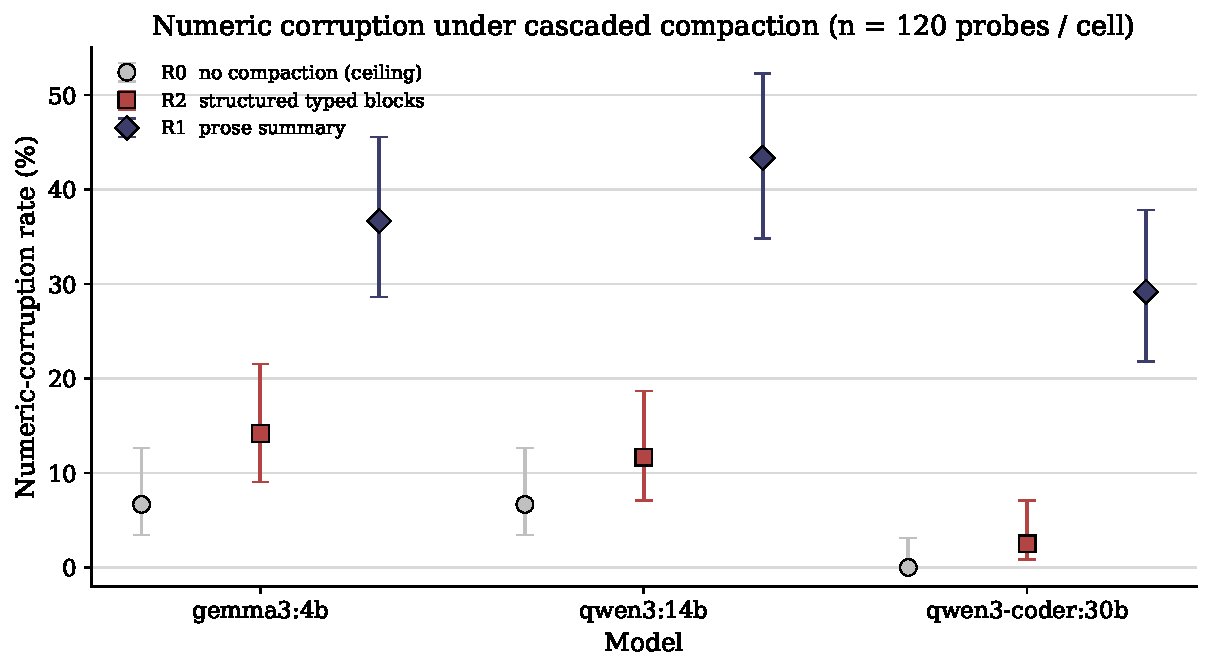
\includegraphics[width=0.78\textwidth]{figures-xr001/fig1-corruption-by-regime.pdf}
\caption{Numeric-corruption rate by model and regime with $95\%$ Wilson
intervals. Ceiling (R0), structured (R2), and prose (R1) are drawn with
distinct colors and markers. In every model the structured point sits near the
ceiling while the prose point sits far above it.}
\label{fig:main}
\end{figure}

\paragraph{Confirmatory test.}
The pre-registered paired exact McNemar test (R1 vs R2 on identical probes),
pooled, gives $b=11$ discordant pairs favoring prose against $c=108$ favoring
structured, two-sided exact $p=3.524\times10^{-21}$. The direction is
R2-better in all three models individually
(Table~\ref{tab:mcnemar}). The falsifier---prose $\approx$ structured at
matched budget---is decisively rejected.

\begin{table}[ht]
\centering
\caption{Paired exact McNemar (R1 vs R2), pooled and per model. $b$: probes
correct under prose but wrong under structured; $c$: correct under structured
but wrong under prose. Direction is R2-better throughout.}
\label{tab:mcnemar}
\begin{tabular}{lcccc}
\toprule
Model & $b$ (R1$>$R2) & $c$ (R2$>$R1) & two-sided $p$ & direction \\
\midrule
Pooled                   & $11$ & $108$ & $3.524\times10^{-21}$ & R2-better \\
\texttt{gemma3:4b}       & $5$  & $32$  & $7.428\times10^{-6}$  & R2-better \\
\texttt{qwen3-coder:30b} & $3$  & $35$  & $6.678\times10^{-8}$  & R2-better \\
\texttt{qwen3:14b}       & $3$  & $41$  & $1.618\times10^{-9}$  & R2-better \\
\bottomrule
\end{tabular}
\end{table}

\paragraph{Matched-budget check.}
Realized compaction budgets are essentially equal: mean
\texttt{eval\_count} of $219.2$ tokens for R1 and $221.4$ for R2 ($180$
compaction calls each, about $1\%$ apart). The measured effect is format, not
budget.

\paragraph{Corruption classes.}
Table~\ref{tab:class} and Figure~\ref{fig:class} give the pooled regime
$\times$ class breakdown. The incident-signature union class
(\texttt{off\_by\_one} $\cup$ \texttt{conflation}) is elevated under prose:
$17$ signature errors for R1 against $4$ for both R2 and R0 ($4.25\times$),
and conflation specifically runs at $16$ for R1 versus $3$ for R2---a
more-than-fivefold elevation. The honest reading, however, is that near-miss
drift is not where
most of the prose deficit lives: R1's error mass is dominated by
\texttt{other\_wrong} $=84$ and \texttt{omission} $=30$, against R2's $25$ and
$5$. Prose compaction mostly \emph{loses} values outright; when it keeps them
near-wrong, it conflates at several times the structured rate.

\begin{table}[ht]
\centering
\caption{Regime $\times$ class breakdown, pooled across models ($n=360$
probes per regime). Signature $=$ \texttt{off\_by\_one} $+$
\texttt{conflation} (the incident-class union, per the pre-registered
precedence).}
\label{tab:class}
\begin{tabular}{lcccccc}
\toprule
Regime & correct & off\_by\_one & conflation & other\_wrong & omission & signature \\
\midrule
R0 & $344$ & $1$ & $3$  & $12$ & $0$  & $4$  \\
R1 & $229$ & $1$ & $16$ & $84$ & $30$ & $17$ \\
R2 & $326$ & $1$ & $3$  & $25$ & $5$  & $4$  \\
\bottomrule
\end{tabular}
\end{table}

\begin{figure}[htbp]
\centering
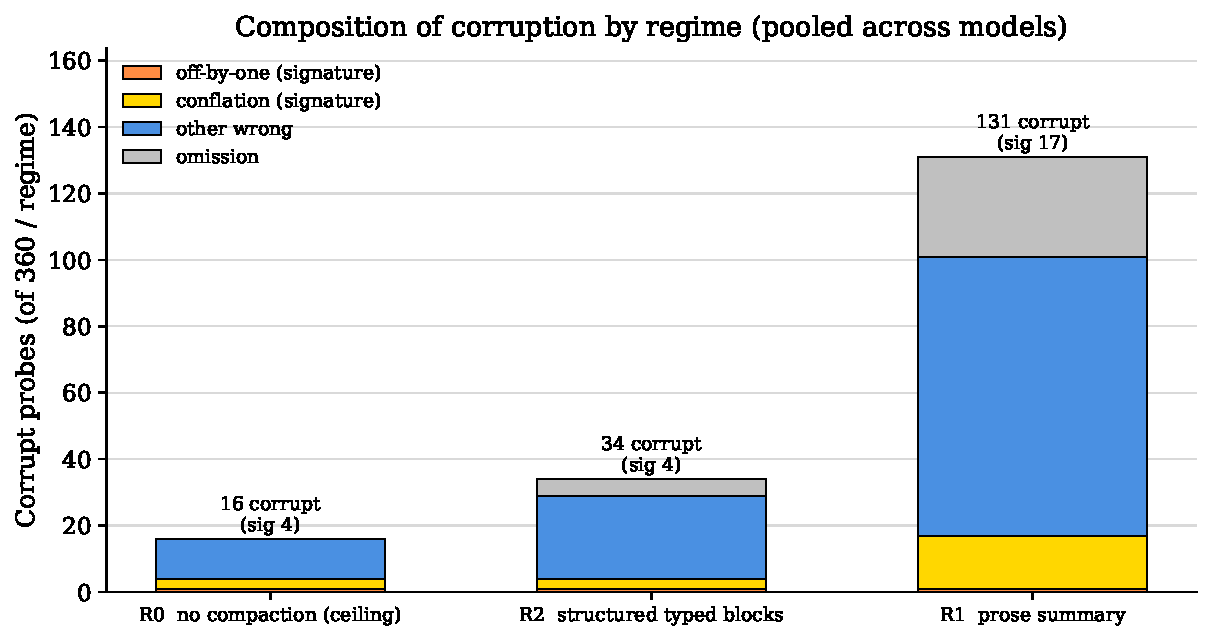
\includegraphics[width=0.78\textwidth]{figures-xr001/fig2-regime-class-breakdown.pdf}
\caption{Composition of the corrupt probes by regime (pooled; correct probes
excluded). The prose bar (R1) is dominated by outright loss
(\texttt{other\_wrong}, \texttt{omission}); the signature near-miss classes
sit at its base and are elevated relative to structured (R2) and ceiling
(R0).}
\label{fig:class}
\end{figure}

\paragraph{Write-time decomposition.}
Parsing the $45$ R1 and $45$ R2 final states and scoring their retained entity
values against ground truth locates most of the prose deficit at write time:
R2 state blocks retain $898/900$ entity values ($99.8\%$), while R1 prose
retains $587/900$ ($65.2\%$). The loss enters predominantly when the summary
is written, not when the question is answered. This metric is exploratory: the
prose side uses the pre-registered nearest-number heuristic, which is crude
and likely understates prose fidelity, and the R2 per-line counter shows a
one-off duplicate-line artifact ($899$ scored correct against $898$ retained);
it carries no confirmatory weight.

\paragraph{Multi-hop completion.}
On the two-entity-sum probes (Table~\ref{tab:multihop}), structured
compaction matches or beats prose in every model, most starkly on
\texttt{qwen3-coder:30b}, where R2 completes $100\%$ against R1's $46.7\%$ (R0
$100\%$). Composing two retained facts is exactly the operation that requires
both to survive compaction with their arithmetic structure intact, and it is
where prose degrades most.

\begin{table}[ht]
\centering
\caption{Multi-hop completion (questions 7--8), the computed sum of two
entities from different segments ($n=30$ probes per cell).}
\label{tab:multihop}
\begin{tabular}{lccc}
\toprule
Model & R0 & R1 (prose) & R2 (structured) \\
\midrule
\texttt{gemma3:4b}       & $73.3\%$  & $30.0\%$ & $50.0\%$  \\
\texttt{qwen3-coder:30b} & $100.0\%$ & $46.7\%$ & $100.0\%$ \\
\texttt{qwen3:14b}       & $73.3\%$  & $20.0\%$ & $53.3\%$  \\
\bottomrule
\end{tabular}
\end{table}

% ===================================================================
\section{Discussion}
\label{sec:discussion}

\paragraph{The loss is a write-time phenomenon.}
The write-time decomposition is the load-bearing observation. Both regimes
answer from a compacted state, both at temperature zero, both under the same
budget; the difference is what survived the act of compaction. Typed blocks
keep almost every value ($99.8\%$) because each value occupies a named slot
that the format obliges the model to fill, whereas prose keeps roughly two of
three ($65.2\%$) because a flowing sentence has no slot that must be filled and
a number that is inconvenient to phrase can simply be dropped or blurred into a
noun phrase. Once a value is gone at write time, no amount of care at read time
recovers it---which is why the prose deficit is dominated by outright loss
rather than near-miss drift.

\paragraph{A rate--distortion reading.}
Compaction is a lossy encoder under a rate budget, and format is the question
of which distortion the encoder may introduce for a fixed rate
\citep{colaco2026ratedistortion}. Prose and typed blocks spend nearly the same
rate here ($219.2$ vs $221.4$ tokens) but incur very different distortion on
the numeric channel: prose lets the encoder trade exact quantities for fluent
connective text, while a typed slot makes the quantity the cheapest thing to
preserve. In Shannon's terms the two formats are different source codes for the
same message at the same rate; the typed code allocates its bits to the tokens
that carry the task. The cascade compounds this---each re-encode is another
chance to drop a value---so a format that has lost a third of its values by
the final checkpoint degrades across the cascade while one that has lost two
in nine hundred barely moves.

\paragraph{Recommendations for agent builders.}
The practical reading is narrow and firm. Give compacted state a typed,
quotable shape---named value slots, explicit combined quantities, explicit
relations---rather than a prose retelling, whenever the state carries numbers
that later steps must recompute against. Do not paraphrase a computed value in
a summary sentence when a \texttt{name: value} line will carry it verbatim.
Treat structure as the compaction format itself, not as an optional garnish on
a prose summary; the measured benefit comes from the format the model is made
to write, and it is largest exactly where agents most need it, on multi-hop
composition of separately stored facts.

\paragraph{Limitations.}
The result rests on one synthetic task family---numeric recall and combination
under filler pressure---chosen to make ground truth exact and the incident
class reproducible; it is not a naturalistic agent workload. The three models
are open-weight, local, span $4$B--$30$B parameters, and duplicate one family
(\texttt{qwen3}); frontier hosted models are untested, so the finding is
claimed only for the measured range. Generation is temperature-$0$
single-sample, so we report no
sampling variance. The compaction budget is a single operating point (about
$120$ words / $256$ tokens); we do not trace the format effect across the
budget curve. The write-time metric's prose side is a heuristic and is
exploratory only. None of these caveats touches the confirmatory McNemar test,
which compares identical probes across regimes within model and so is immune to
task-difficulty, model, and episode confounds.

\paragraph{What the result does not claim.}
We make no claim about semantic or narrative content: prose may well preserve
intent, rationale, or discourse structure that a typed block discards, and
this experiment does not measure that. We make no claim about model internals
or mechanisms of representation. And we do not claim the hypothesis is
novel---that numbers are fragile under summarization, and that structure
preserves them, is the explicit position of the flanking work in
Section~\ref{sec:rw}. The claim is bounded to numeric state: at matched token
budgets, under cascaded compaction, the format the LLM writes changes numeric
corruption from roughly one fact in three to under one in ten.

% ===================================================================
\section{Reproducibility}
\label{sec:repro}

Everything needed to reproduce the result is public in the rhombic repository
(\url{https://github.com/tasumermaf/rhombic}) under
\texttt{results/XR-001-externalization-pilot/}: the pre-registered protocol
with its dated amendment (\texttt{PROTOCOL.md}), the seeded episodes and their
ground truth (\texttt{tasks.json}; base seed $77001$, episode seed $=$ base
$+$ index), the run ledger (\texttt{manifest.json}), every LLM call with full
prompt, response, token counts, and timing (\texttt{raw/}), the scored
probe-level records (\texttt{results.json}), and the generated analysis
(\texttt{analysis.md}, \texttt{RESULTS.md}). The runner
(\texttt{scripts/xr001\_externalization\_pilot.py}) is standard-library-only,
speaks to the Ollama HTTP API at \texttt{localhost:11434}, and updates its
manifest after every episode so the sweep is safe to interrupt and resume; the
manifest records the tasks-file SHA-256 and refuses to resume against a
different task set. Protocol, runner, and pre-launch amendment were committed
at \texttt{e2aa6fc}; two post-freeze runner guards (manifest hardening, no
metric changes) landed by \texttt{bae4079}, the state the run executed; the
confirmatory analysis is committed at \texttt{a777adb}. The run reported here
used
three local Ollama models on a single consumer laptop GPU (RTX 4090 Laptop,
$16$ GB) at $\$0$ marginal cost; wall time was $84$ minutes. Figures are
regenerated deterministically from \texttt{results.json} by
\texttt{paper/figures-xr001/make\_figures.py}.

% ===================================================================
\section*{Acknowledgments}
Experimentation, analysis, and drafting were performed with a standing AI
research collaborator (Claude, Anthropic); all numbers reported here were
machine-verified against the frozen artifacts rather than restated from any
model's summary.

% ===================================================================
% --- references ---
\bibliographystyle{plainnat}
\bibliography{rhombic-xr001}

\end{document}
